\chapter{Evaluation}
\label{cha:evaluation}

To prove the project's usability, it has not only to be tested against a ``real'' setup; additionally, it also has to be tested against different settings. Since it was designed to be as unopinionated as possible, there are still challenges to face concerning the overall support of different third-party tools, like template engines, etc\ldots

Nevertheless, a base repository for future building using the REST API is set up without much hassle. As the project features a generic Metalsmith instance building and rendering the different website projects, a local installation setup might as well be useful prior to handing the repository over to the REST API. This might help in fixing bugs, which are probably much easier detected, if the source code is at hand.

\section{Minimal requirements}
\label{sec:minimalrequirements}

For even being able to build a repository successfully, it has to consist of a ``valid'' Metalsmith project. This means, that a few requirements have to be met, such as the following:

\begin{itemize}
  \item A folder structure, which consists of at least a source folder inside the project root,
  \item a configuration file, either in YAML or JSON format and named \emph{\_config.*},
  \item and finally being hosted on GitHub as public repository.
  \item Furthermore, it must not rely on any other build tools (e.g. \emph{Gulp}\footnote{\url{http://gulpjs.com} -- Website of Gulp.js}, \emph{Webpack}\footnote{\url{https://webpack.js.org} -- Website of Webpack.}, etc\ldots), only Metalsmith is supported at this time.
\end{itemize}

\subsection{Configuration file}
\label{sec:minimalrequirements-configuration}
The configuration file is probably the most critical part in the repository's contents, as it is the only source for the build pipeline to obtain the setup instructions from. Since the Metalsmith CLI is able to render a project based on a single JSON configuration file and the API setup doesn't really differ, the format of the configuration needed by the REST API is nearly identical. Therefore, the configuration for a local Metalsmith installation and the one used for the project's build pipeline are very well interchangeable (see Program \ref{list:pipeline-config}).

\begin{program}
  \caption{\textbf{\_config.yml} -- a sample configuration file, containing some global configuration data, as well as a few Metalsmith plugin definitions.}
  \label{list:pipeline-config}
\lstinputlisting[language=ruby]{chapters/06-evaluation/_support/_config.yml}
\end{program}

Since the REST API is able to parse both YAML and JSON notations, it is up to the developer to choose what fits his/her needs best. Since Metalsmith only understands JavaScript, any YAML configuration is parsed to JSON by the API, prior to forking the child process. This makes sense in a way, as the build setting information is getting included in the general options object, which is handed over from the REST API to the build pipeline, where parts of it get stored in the database together with the build log.

\subsection{Local testing}
Having a local Metalsmith install at stake may not only support the developer in finding and fixing bugs, it also helps to constantly pursue a clean build setup. The remote build pipeline neither is configured to inform about any installed modules, nor is it able to independently draw any conclusions of the provided configuration file. The only way to communicate with any responsible developer, is to send E-Mails containing status messages, or to respond build log information from the database upon request.

Although caching is not available when testing locally, it is often the only way to fix the build tree in a way, that Metalsmith is able to produce a successful outcome again. The reason behind that is the fact, that developers often try to fix a bug using subsequent small code changes -- this requires multiple rebuilds to check if the effort succeeded. However, it is also possible to patch the code base by adding one commit after another and analyze the messages of the build log entries.

\section{Comparison}
\label{sec:comparison}

When trying to compare the project's build pipeline to standalone static site generators like Jekyll or Metalsmith, it has to be stated, that neither one of those requires a git repository, nor any sort of authorization (besides during their installation process possibly). Furthermore, Jekyll also provides a command line argument for setting up a base project (see ch. \ref{sec:jekyll-technology} on p. \pageref{sec:jekyll-technology}), so that hardly any time is lost before a content author actually is being able to start writing.

As this project initially was designed to support porting Jekyll projects to Metalsmith, it already requires a basic structure for being able to work with. However, when starting from scratch, the probably best advice is to set up a local project, which makes use of the Metalsmith CLI and then start porting the configuration to fit the REST APIs standards.

\subsection{Jekyll}
A Jekyll project, as already explained in ch. \ref{sec:jekyll-technology}, is entirely written in Ruby and sets up on the Liquid templating engine. As a configuration file, it requires a YAML file called \emph{\_config.yml} in the project root and supports parsing data from YAML, JSON and CSV files to usable site variables out of the box \cite[76]{dhillon2016}. A functional Jekyll project also has to be equipped with Liquid templates in the \emph{\_layouts} folder, together with a few more directories holding different contents resulting in various recycleable parts during the build process. As of Jekyll 3.2, most of these parts have gotten outsourced in different Ruby gems, thus being hidden to the public and making it harder to port them to other generator applications like Metalsmith \cite{JekyllDirectoryStructure}.

\subsubsection{Jekyll source repository}
Parallel to the development of this project, the Jekyll docs sources\footnote{\url{https://github.com/jekyll/jekyll/tree/master/docs} -- Jekyll docs section in the Jekyll repository on GitHub.} were ported the best possible for setting a benchmark for the usability of the REST API. To make this happen, a few major changes needed to be made in order to get a positive build result:

\begin{itemize}
  \item The root folder was put in the source folder, but \emph{\_data}, \emph{\_layouts} and \emph{\_includes} were left out. Additionally, all asset-containing folders were moved into the \emph{\_public} directory.
  \item Necessary plugins were installed and configured for correctly setting the render flow:
  \begin{itemize}
    \item metalsmith-date-in-filename,
    \item metalsmith-sass,
    \item metalsmith-collections,
    \item metalsmith-permalinks,
    \item and a few more\ldots
  \end{itemize}
  \item Due to the limitations of \emph{TinyLiquid}\footnote{\url{https://github.com/leizongmin/tinyliquid} -- TinyLiquid repository on GitHub.}, especially file paths in include and extend statements had to be adjusted.
  \item Some functionality still does not work without further engineering, for example the YAML files in the \_data directory, or gem-dependent tasks like generating the sitemap or managing redirects.
\end{itemize}

To conclude; it is possible to successfully render a Jekyll project using Metalsmith, although there are a lot of adjustments necessary beforehand, not to speak of the deficits of the TinyLiquid package. Therefore, the expected behaviour of the outcome is likely to differ heavily from the reality. The test repository for this evaluation was obviously uploaded on GitHub\footnote{\url{https://github.com/vorchdorfmedia/jekyll-docs} -- Test repository for porting a Jekyll project to Metalsmith.} and may be tested locally using the Metalsmith CLI.

\subsection{Metalsmith}
Since Metalsmith was chosen for use as static site generator within the REST API (see ch. \ref{sec:primarythoughts-generator} on p. \pageref{sec:primarythoughts-generator}), it should be used as the foundation framework for any website project, which should be built using the REST API in the future. Due to the fact that Metalsmith is yet another npm module built for Node.js, it also offers to act as part of any available build tool, such as Gulp, Webpack or else -- however, this is not supported (see ch. \ref{sec:minimalrequirements} on p. \pageref{sec:minimalrequirements}).

The main reason behind this limitation is, that automatically detecting a different or additional build setup is error-prone and may easily slow down the render process. Furthermore, Metalsmith offers a feature-rich API and the possibility of writing plugins\footnote{\url{http://www.metalsmith.io/\#writing-a-plugin} -- ``Writing a plugin'' section in Metalsmith's documentation.} to fit the developer's needs, thus making nearly any additional build tool obsolete. All that is left to do, is to publish any written plugin publicly available to npm and append it to the repository's configuration file for future use in the build pipeline. As a result, other developers may also download and/or enhance the plugin to keep it up to date.

\section{REST API}
\label{sec:restapi}
The REST API was built and designed as remote-acting standalone web application, running on Node's servers-side JavaScript engine. Apart from specificly reserved firewall ports, the project is only dependent on a Node.js install, every other dependency may be installed using npm, regardless on the used operating system.

By extending any desired Node.js Dockerfile\footnote{\url{https://hub.docker.com/\_/node/} -- Official repository for Node.js on Docker Hub.}, it may be even run as autonomous Docker container and therefore multiplied for better load balancing based on the current HTTP load extent.


%% Screenshot of console log output after running artillery
\begin{figure}[h] % h-ere, t-op, b-ottom, p-age
    \centering
    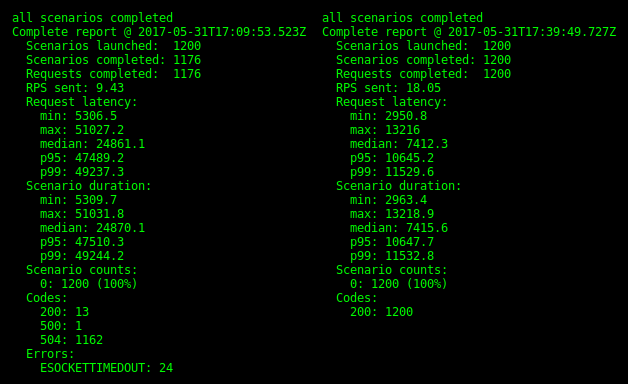
\includegraphics[width=0.9\textwidth]{pen_test.png}
    \caption{Screenshots of two command line outputs showing the results of the REST API being put under high HTTP load. During 60 seconds, the API had to face \emph{1200 requests} of 20 virtual clients created by Artillery. The test on the left was defined to include a single POST request triggering a new build cycle (with a full rebuild option) every time the API accepted a new connection. The results show the following: \emph{24} could not be handled at all, \emph{1162} resulted in gateway timeouts (GitHub blocks), but \emph{13} were handled successfully and returned with a \emph{200 OK} HTTP status code.}
    \label{fig:pen-test}
\end{figure}
%

%% Screenshot of the Mailgun result log
\begin{figure}[h] % h-ere, t-op, b-ottom, p-age
    \centering
    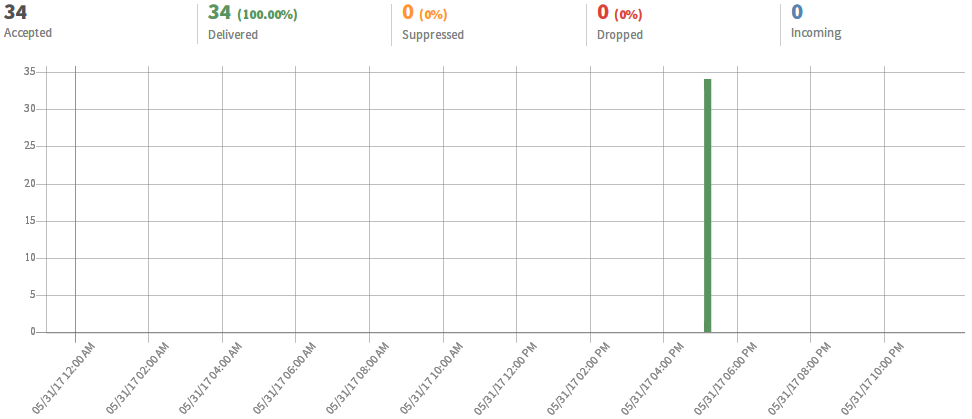
\includegraphics[width=0.9\textwidth]{mailgun_result.png}
    \caption{A screenshot showing the extent of the previous load-test (see fig. \ref{fig:pen-test}) in the Mailgun dashboard. Obviously, the build pipeline was triggered \emph{34} times, leading to the same number of E-Mails being sent. Out of this 34 E-Mails, \emph{8} showed a success message, whereas the others mostly failed due to other concurrent requests deleting the CWD as a preparation step prior to downloading the repository archive.}
    \label{fig:mailgun-result}
\end{figure}
%

\subsection{Load testing}
To evaluate the basic stability while handling multiple concurrent requests, the API was put under a high load test using Artillery\footnote{\url{https://artillery.io} -- Website of Artillery, a load testing toolkit.} (see fig. \ref{fig:pen-test}). Without any load balancing, nor any other high load supporting tool, 1200 POST requests triggered the build pipeline for a total duration of 60 seconds. As explained in the graphic's caption, the penetration test showed a success rate of roughly 1\%, a reasonable minimal response time of about 5 seconds but a terrible maximum response time of 51 seconds.

Of course, this data may not be interpreted as successful result in the first place, but it has to be stated, that the test was run on the endpoint causing the heaviest task in the system and most failure responses were effected by GitHub blocking most requests due to their rate abuse checking system.

The same test running on a much lighter task is showing a different picture; 1200 GET requests for receiving information about the latest build cycle had a response rate of 100\%. The response time ranged from 3 to 13 seconds, which is again a sign to not let a single application handle such an amount of requests without load balancing beforehand. In the end, it is safe to say, that the REST API may handle a reasonable amount of requests quite well on its own (e.g. requests triggered by GitHub webhooks), but consisting of multiple instances may be the best option for handling a significant amount of requests every once in a while.

